\documentclass[10pt,twocolumn]{article}

% use the oxycomps style file
\usepackage{oxycomps}

% usage: \fixme[comments describing issue]{text to be fixed}
% define \fixme as not doing anything special
\newcommand{\fixme}[2][]{#2}
% overwrite it so it shows up as red
\renewcommand{\fixme}[2][]{\textcolor{red}{#2}}
% overwrite it again so related text shows as footnotes
%\renewcommand{\fixme}[2][]{\textcolor{red}{#2\footnote{#1}}}

% read references.bib for the bibtex data
\bibliography{references}

% include metadata in the generated pdf file
\pdfinfo{
    /Title (Music Plug-in in C++ tutorial report)
    /Author (James Wang)
}

% set the title and author information
\title{Music Plug-in in C++ tutorial report}
\author{James Wang}
\affiliation{Occidental College}
\email{jwang2@oxy.edu}

\begin{document}

\maketitle

\section{Introduction}

In my computer science senior comprehensive project, I am exploring the field of music technology with the aim of developing accessible music creation software, which targets individuals who are novices in music production, with the core objective of democratizing music production. Users are empowered to create harmonies, rhythms, melodies, and explore basic production techniques, such as using equalizers and compressors. 
The project is underscored by two major technical components. The first is an accessible and educational user interface, designed to accommodate users of varying musical backgrounds with ease. The second aspect revolves around the knowledge of digital signal processing skills. The tutorial is based on the JUCE framework, which stands out as a comprehensive C++ package for developing audio plugins. It not only provided a basic interface design using the JUCE framework in C++, but, more crucially, it laid the foundational knowledge for the second goal. 

\subsection{Tutorial Overview}
The tutorial\cite{YouTubeVideo2023} I embarked upon guides me through the process of building a 3-band equalizer using modern C++ and the JUCE Framework. This experience is crucial, as the ability to manipulate audio through equalization is fundamental to achieving sound shaping required by the software. The creation of this 3-band equalizer not only familiarizes me with essential signal processing concepts but also sets the stage for the development of more complex audio effects and instruments. Mastering the development of such plugins is vital for incorporating post-production audio effects and sound sources, including virtual studio technology (VST) instruments and effects, into the software. This tutorial is directly aligned with the overarching goal of my project: to simplify the music production process for non-musicians, while still offering the depth needed to produce high-quality, creative soundscapes.

\subsection{Objectives}
A successful outcome for this project extends beyond the technical feat of software development. At its heart, success is defined by the software's ability to present an accessible, intuitive user interface while retaining the sophistication needed to shape sound according to the user's desires. This involves real-time visual feedback, such as a spectral analyzer that dynamically responds to adjustments in parameters, offering users immediate insights into the impact of their creative decisions. Moreover, a successful outcome would also encompass the software's ability to inspire creativity among users, providing a seamless blend of guided processes for music creation and the flexibility to experiment and explore sonic possibilities. Thus, the tutorial's relevance and the project's ambitions coalesce into a singular vision: to empower individuals to express their musical creativity, unfettered by the complexities of traditional music production tools.


\section{Methods}

The methodology underlying the development of a 3-band equalizer plugin involves a detailed, step-by-step approach, leveraging the JUCE framework. It is essential to acknowledge the fundamental concepts central to this tutorial: an equalizer (EQ) and a plugin. An EQ is an audio processing tool that allows the manipulation of the frequency balance of an audio signal, enhancing or attenuating specific frequency bands according to the user's preferences. A plugin, in this context, refers to software that adds specific capabilities to a host application, such as a digital audio workstation (DAW). This project focuses on developing an Audio Unit (AU) plugin format, which is compatible with various DAWs on macOS, including GarageBand, Logic, and Ableton, alongside other formats like VST/VST3 and AAX, catering to a broad spectrum of production environments. This plugin is designed as a stereo plugin, to process two channels of audio (left and right) simultaneously, contrasting with a mono plugin that processes a single audio channel, thus allowing for the manipulation of spatial audio properties. To ensure flexibility and access to a wide array of features, the JUCE framework was set up with Git, enabling the reference to older versions of the framework, thus facilitating a more controlled development environment.


\subsection{Initialize Parameters}
The development process began with the creation of audio parameters using the Audio Processor Value Tree State in the JUCE framework. This component is instrumental in managing plugin parameters, facilitating the smooth integration and automation of parameters within DAWs. The EQ features include a high-pass filter with adjustable slope and frequency(as shown in figure 1 left column), a band-pass filter with modifiable Q (quality factor), frequency, and gain(figure 1 middle column), and a low-pass filter with configurable slope and frequency(figure 1 right column), catering to a wide range of audio sculpting needs.

\subsection{Digital Signal Processing}
The Digital Signal Processing (DSP) setup involved a detailed process of meticulously defining each filter's functionality—how they attenuate or amplify certain frequency bands, thereby shaping the audio signal's tonal quality. This process starts by configuring a stereo buffer to handle audio processing for two channels simultaneously, reflecting a  stereo experience by allowing independent processing of left and right audio signals. Then, I identify the type of each filter—whether high-pass, band-pass, or low-pass in determining how they interact with the audio signal. This classification facilitated a structured approach to manipulating frequency bands, where each filter type was tailored to target specific aspects of the audio spectrum. High-pass filters were set to eliminate lower frequencies below a certain threshold, band-pass filters to isolate a particular frequency band, enhancing or attenuating it, and low-pass filters to remove high frequencies above a certain point. Furthermore, the integration of these filters with the corresponding audio parameters through the audio processor value tree state was a critical step, bridging the gap between the user interface and the underlying audio processing. Connecting parameters. This seamless connection ensures that the plugin responds dynamically to user interactions, providing an intuitive and interactive experience that reflects changes in real-time.



\subsection{Graphic User Interface}
The development of the Graphical User Interface (GUI) underwent significant enhancements with a focus on improving usability. Adjustments to the color scheme and structural layout were implemented to ensure that the software not only remains intuitive for users to control the 3-band equalizer's parameters via sliders and knobs but also becomes visually engaging, further enhancing the user experience. Leveraging the basic JUCE interface package, the GUI revisions were aimed at embodying a blend of simplicity and visual appeal, making it easier for users to navigate through the plugin's features. Each parameter control on the interface was meticulously re-evaluated and adjusted, ensuring that user interactions would yield immediate  effects on the sound output, thus promoting a more immersive and tactile learning experience.

However, it's important to acknowledge that in this phase of development, comprehensive instructions and a written tutorial specifically designed for non-musicians were not integrated within the GUI. The potential learning curve for individuals without formal musical training is recognized as a critical aspect of the software's accessibility. As such, there is a committed plan to devote attention to the creation of these educational resources in the future iterations of the software. The goal is to include step-by-step instructions and tutorials directly within the software environment, offering users clear guidance on exploiting the plugin's full capabilities. This approach is intended not just to clarify the technicalities of music production but also to empower users, fostering confidence in their ability to experiment and craft music creatively. 


\begin{figure}
    \centering
    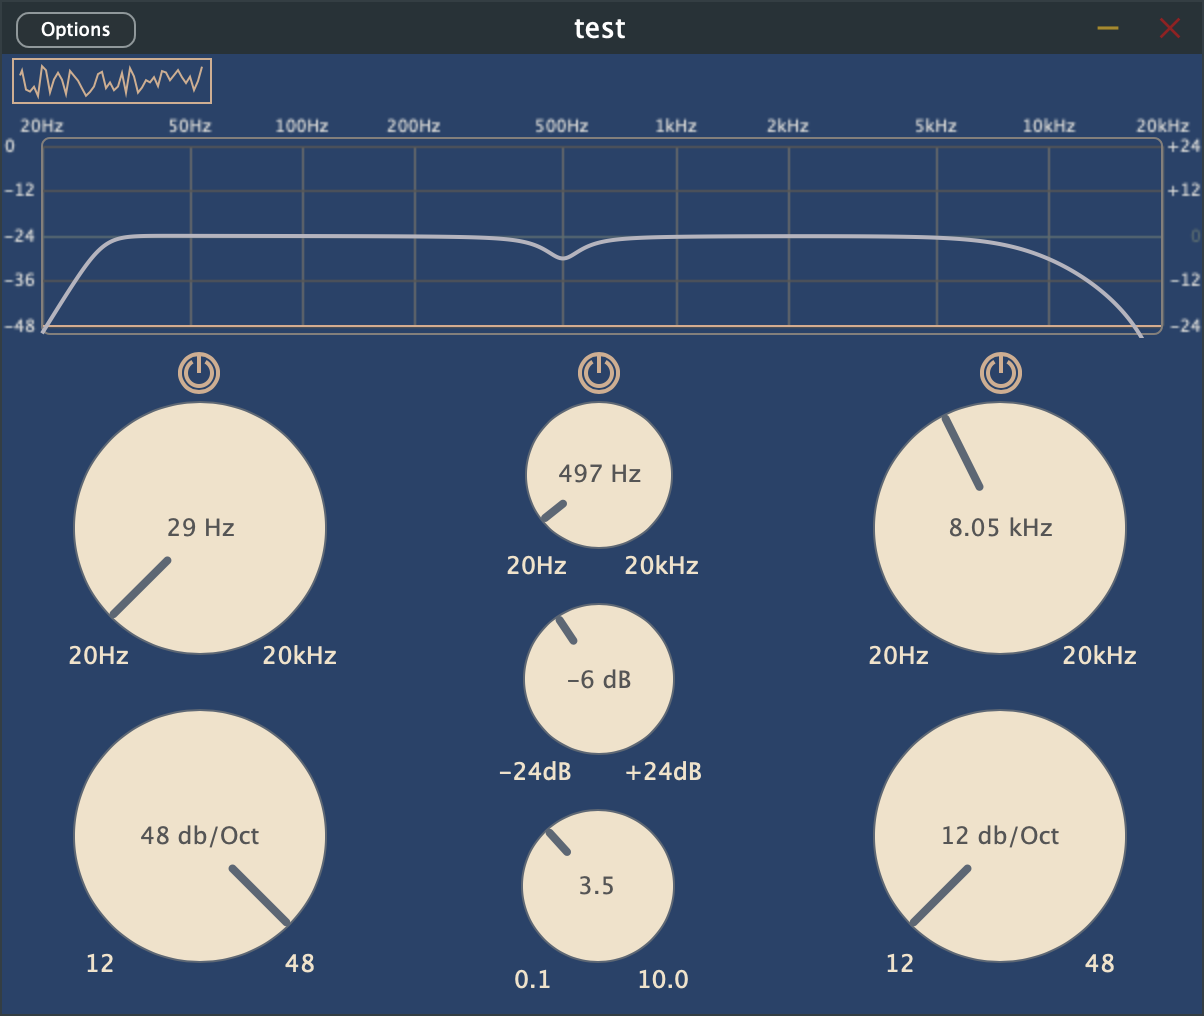
\includegraphics[width=.95\linewidth]{GUI.png}
    \caption{
        the User Interface
    }
    \label{fig:first-page}
\end{figure}
\subsection{Spectrum Analyzer}
The spectrum analyzer is a cornerstone of the plugin, offering a sophisticated visualization of the audio's real-time frequency spectrum. This powerful feature is brought to life by processing the audio signal in predetermined blocks, analyzing these blocks to generate Fast Fourier Transform (FFT) data, which is then  rendered through a spectrum analyzer. The inclusion of this functionality is crucial, as it enables users to visually track the audio signal's frequency content, significantly enhancing both the educational and practical value of the plugin.

By providing a visual representation of how sound frequencies are distributed by adjustments within the plugin, the spectrum analyzer plays a vital role in demystifying the often complex domain of digital signal processing for the user. This visualization is not just a tool for expert analysis; it is designed with accessibility in mind, making the software more approachable for individuals with varying levels of musical knowledge and production experience. The spectrum analyzer helps bridge the gap between abstract audio concepts and tangible user actions, allowing users to see the immediate impact of their adjustments on the sound's frequency spectrum. This direct feedback loop aids in fostering a deeper understanding of the software's capabilities, encouraging users to explore and experiment with different settings confidently.


\subsection{Conclusion}
In conclusion, the comprehensive knowledge and experience garnered through this project, from setting up the JUCE framework to integrating complex DSP operations and developing an intuitive GUI, lay a solid foundation for the successful completion of my senior comprehensive project. This endeavor not only sharpens my technical acumen in audio software development but also enriches my understanding of audio signal processing, ultimately facilitating the creation of accessible music creation software that embodies the principles of user-friendliness and advanced audio manipulation capabilities.


\begin{figure}
    \centering
    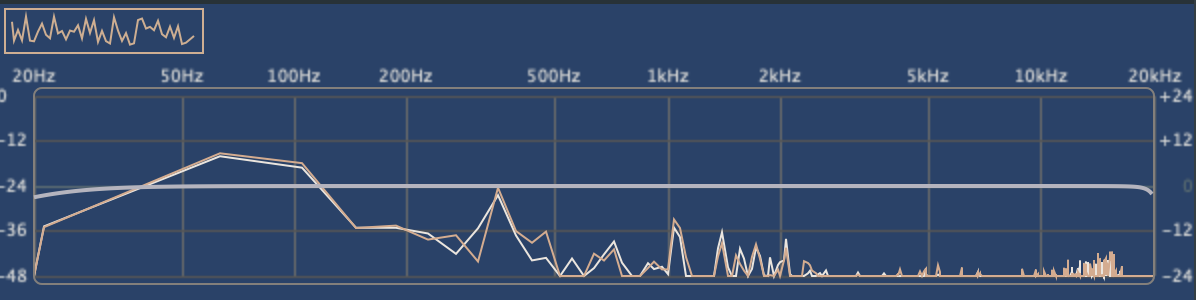
\includegraphics[width=.95\linewidth]{spectrum analyzer.png}
    \caption{
        the spectrum analyzer
    }
    \label{fig:first-page}
\end{figure}


\section{Metrics and Evaluation}
The effectiveness and usability of the 3-band equalizer plugin, especially in the context of its accessibility and learning capabilities for non-musicians, necessitate a methodical evaluation approach. The proposed metrics for this evaluation involve a combination of quantitative and qualitative analyses through user interviews and practical usage assessments. The evaluation plan aims to engage two distinct user groups: music production students and non-musicians, each offering unique insights into the plugin's design and educational value.

\subsection{For Music Students}
For music production students, the primary quantitative metric is the time required to achieve mastery in utilizing the plugin for a predefined task, such as mixing a given song. This measure will provide a direct indication of the plugin's learnability and efficiency in a professional context. Complementing this, qualitative feedback will be collected through structured interviews focusing on the students' perceptions of the interface's intuitiveness, effectiveness, and any suggestions for improvement. This dual approach aims to uncover not only the plugin's practical utility in a music production environment but also its ergonomic design and user experience satisfaction levels.

\subsection{For Non-musicians}
Conversely, for non-musicians, the evaluation shifts towards a more exploratory and qualitative framework. After a period of interaction with the plugin, participants will be interviewed to gauge their experiences, particularly how the plugin facilitated their understanding of audio processing and whether the visual and auditory feedback mechanisms (e.g., the response curve grid and spectrum analyzer) effectively conveyed the impact of their adjustments. Questions will also explore the ease with which users could discern audio changes, thereby assessing the plugin's educational potential and its ability to demystify music production concepts for beginners.

\subsection{Limitations}
It's important to note that, due to time constraints, the outlined evaluation plan remains a prospective endeavor, with its execution slated for after the completion of the software development phase. This forward-looking approach underscores the project's commitment to iterative improvement and user-centered design. By engaging with both experienced and novice users, the evaluation aims to refine the plugin's usability and educational value, ensuring it meets the diverse needs and learning curves of its intended audience.

In anticipation of this evaluation, this project acknowledges the critical role of user feedback in guiding subsequent revisions and enhancements. The insights garnered from this two-pronged evaluation will be instrumental in tailoring the plugin not only to facilitate creative expression among non-musicians but also to streamline the music production process for professionals, thereby bridging the gap between technical complexity and artistic exploration.



\section{Reflection}
Embarking on this tutorial to develop a 3-band equalizer plugin using the JUCE framework has been a transformative journey in my understanding of low-level audio software development. This tutorial has illuminated the intricacies of the JUCE framework, which was previously a domain I had only superficially engaged with. Prior to this, my vision for the senior comprehensive project was to create standalone music creation software, primarily utilizing the Qt framework for its development. However, the insights gained from this tutorial have expanded my perspective, revealing the potential for integrating my project within modern Digital Audio Workstations (DAWs) as a plugin.

This realization marks a significant shift in the scope and potential impact of my project. By adopting the plugin approach, the software could reach a broader audience, providing value to users within their preferred music production environments. This integration could enhance the usability and accessibility of the tool, allowing users to leverage its features alongside other plugins and tools within DAWs.

However, this expanded vision comes with its challenges. The tutorial has highlighted my need for a deeper dive into the JUCE framework to fully harness its capabilities for developing sophisticated audio processing tools. While I have gained a foundational understanding of audio parameter manipulation, DSP (Digital Signal Processing) setup, and GUI (Graphical User Interface) development, I recognize the necessity of investing significantly more time into mastering the JUCE framework. This entails not just a technical understanding but also an appreciation for the framework's architectural nuances and best practices for plugin development.

\printbibliography

\end{document}
